\chapter{Quantum Physics Background}\label{ch:qm_background}

\begin{figure}[h]
    \centering
    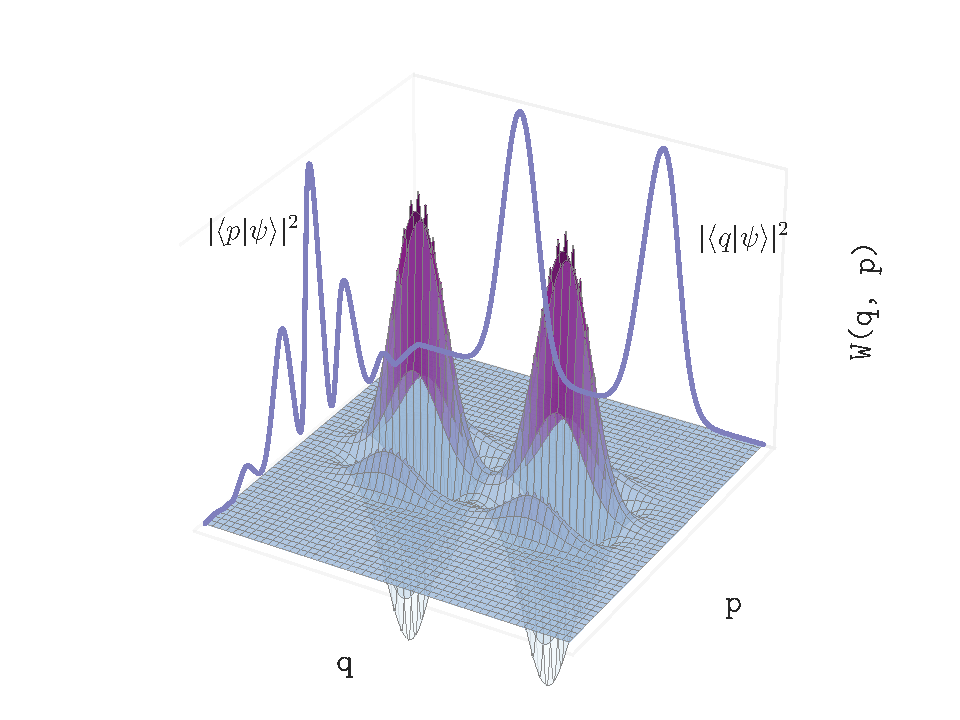
\includegraphics[width=0.8\linewidth]{Chapters/Theoretical_Background/images/QM_section_cover.pdf}
    \caption{Wigner quasi-probability function $W$ as function of position $q$ and momentum $p$.}
    \label{fig:QM_section_cover}
\end{figure}

%=============================================================
\section{Basic Linear Algebra background}
\subsubsection{Dirac Notation and Completeness}
We start with a basic review of linear algebra for two main reasons. First, we want to emphasise that from the beginning we are dealing with complex n-dimensional vector spaces, sub-spaces of $\mathbb{C}^n$, so that an element $\mvec{z} \in \mathbb{C}^N$ can be represented as an n-tuple $(z_1, z_2, ..., z_n)$ where $z_i$ is a complex number. Second, we want to migrate to the standard Dirac notation as soon as possible, showing what it means and why we are doing it.

Using the Dirac notation, we represent a standard basis for the vector space $\{e_i\}$ with ket vectors, written as $\{\ket{i}\}$, with $i \in \mathbb{N}$. A generic vector $\ket{a}$ in this space can be decomposed in terms of a complete basis as
\begin{align*}
    \ket{a} =  \sum_i \ket{i}a_i = \sum_i \ket{i}\bra{i}\ket{a}.
\end{align*}

In the second equality, the completeness of the basis is apparent, which can be represented as 
\begin{align*}
    I =  \sum_i\ket{i}\bra{i},
\end{align*}
with $I$ being the identity matrix. This completeness relation is crucial in quantum mechanics because it guarantees that the basis spans the entire vector space, allowing the decomposition of a general $\ket{a}$.

\subsubsection{Operators and Adjoint Operators}
A linear operator $\op{O}$ is a mathematical object that maps one vector to another. We say it ``acts'' on a vector $\ket{a}$, returning another vector, as in $ \op{O}\ket{a}=\ket{b}$. We can also define the adjoint of this operator as the operator that maps the dual \cite{curtis2012linear} of vector $\ket{a}$ to the dual of vector $\ket{b}$. In Dirac notation, this can be written $ \bra{a} \op{O}^\dagger =\bra{b}$. Furthermore, in quantum-mechanical contexts, the dual of the ket vector is called a bra vector, and we denote it $\bra{a} = \ket{a}^\dagger$. This way, an inner product is written $\bra{a}\ket{b} \coloneqq \braket{a}{b}$.

For an operator to be called linear, it must obey the following linearity property:
\begin{align*}
    \op{O}(x\ket{a} + y\ket{b}) = x\op{O}\ket{a} + y\op{O}\ket{b},
\end{align*}
where $x,\,y$ are scalars. One fundamental aspect of linear operators is that, given a choice of a basis $\{\ket{i}\}$, we can represent them as matrices. Thus, the linear transformation can be viewed as a matrix-vector multiplication: 
\begin{align*}
    \op{O}\ket{i} = \sum_{j} \ket{j}O_{ji}.
\end{align*}

To obtain the matrix elements of the matrix representation of the operator $\op{O}$ we can consider the inner product of different basis vectors:
\begin{align*}
   O_{ki} = \bra{k}\op{O}\ket{i} = \sum_{j} \braket{k}{j}O_{ji},
\end{align*}
where $\ket{k}$ and $\ket{j}$ are basis vectors in the vector space on which $\op{O}$ acts. The subsequent application of linear operators can similarly be expressed as subsequent matrix multiplications, which means that if $\op{C} = \op{A}\op{B}$, then
\begin{align*}
C_{ij} = \sum_k A_{ik}B_{kj}.
\end{align*}

From that it is clear that $\op{A}\op{B} \neq \op{B}\op{A}$ in general. This distinction can seem obvious, but deserves special attention for its implications in quantum mechanics. Let us define the commutator of operators:
\begin{align*}
    [\op{A},\, \op{B}] = \op{A} \op{B} - \op{B}\op{A}.
\end{align*}

When the commutator of two operators is zero, they are said to commute with each other.

\begin{JTD}
\footnote{Since we are assuming some prior knowledge, we introduce these boxes, in which we connect what is presented with not yet defined concepts. This is a clear compromise in linearity of narrative to make the reading more interesting for those with prior knowledge.}When two operators commute,
    \begin{itemize}
        \item the sequence of measurements does not affect the result;
        \item it is possible to find states that are eigenstates for both operators, meaning we can know the outcome for both measurements precisely and simultaneously;
        \item if an operator commutes with a special operator we call the Hamiltonian ($\hat{H}$), it can be associated with a conserved physical quantity.
    \end{itemize}
\end{JTD}

\subsubsection{Additional Matrix Properties}
Linear algebra is the language of quantum mechanics. As such, there are several properties of matrices that need to be mentioned, even if they seem to appear with no motivation for now.
\begin{itemize}
    \item \textbf{Hermitian Matrices:} If a matrix $A$ is such that $A^\dagger = A$, it is called Hermitian. In quantum mechanics, this is relevant because every observable can be represented by a Hermitian operator. 
    \item \textbf{Unitary Matrices:} If a matrix $A$ is such that its inverse is equal to its adjoint ($A^{-1} = A^{\dagger}$) it is called a unitary matrix. This is relevant because unitary operators preserve the inner product ($\langle Ax, Ay\rangle =\langle x, y\rangle $) and vector norms. Consequently, they preserve probability amplitudes.
    \item \textbf{Orthogonal Matrices:} A unitary matrix with real elements is called orthogonal. They are important because they represent transformations that do not break the orthogonality of vectors - a crucial point in coordinate transformations.
\end{itemize}

\subsection{Hilbert spaces}
Quantum and classical mechanical states are different conceptual objects. Unlike a classical state, a general quantum state \textbf{needs} to be represented as elements of a vector space known as a Hilbert space. In Newtonian mechanics, the vector spaces used are Euclidean. In contrast, Hilbert vector spaces have some major differences.

First, Euclidean vector spaces are vector spaces over the real numbers, while Hilbert spaces are more generally defined over the complex field.
Additionally, Euclidian spaces are finite-dimensional, whereas Hilbert spaces generalise the idea of an inner product to infinite dimension.
Finally, Hilbert spaces require us to be more precise with the concept of sequence convergence. In particular, a Hilbert space must be Cauchy-complete. Intuitively, this means that every sequence that ``seems like'' it should converge (to another element of the space) in fact does. 

This third difference is more subtle because we get it for free in Euclidian spaces \cite{rudin}, and thus, it does not often cross our minds - Euclidian spaces inherit Cauchy completeness from the real numbers.

We do not intend to be rigorous in our definition of a Hilbert space, and a complete discussion is found in \cite{rudin}. We care about the convergence of sequences because we want to use calculus in this vector space, and, therefore, limits have to be well defined. Furthermore, we often want to expand quantum states as an infinite sum of eigenvectors of an observable, again requiring a precise definition of limits.

\subsection{From Euclidian vectors to functions}
In this section, we transition from Euclidian vectors to function spaces. Some function spaces can also be vector spaces, so we must define analogous properties for this type of space to be mathematically consistent. Using the previous formalism, we can express the orthonormality of basis vectors as 
\begin{align*}
    \braket{i}{j} = \delta_{ij} \coloneqq \begin{cases}
        1, \enspace i=j\\
        0  \enspace\enspace \text{else},
    \end{cases}
\end{align*}
where $\delta_{ij}$ is called the Kronecker delta. 

\subsubsection{Orthogonality in function spaces}
Function spaces, however, may have an infinite-dimensional basis, which means that they require an infinite number of basis functions to span the space. Because of that, the inner product becomes an integral. For Euclidian vectors, operations combine point coordinates via some rule, such as addition. However, the image of a function ``points to'' many points at once, possibly infinitely many. Therefore, the idea of an inner product is naturally extended by the integral over a function multiplied by its dual.

Consider the (enumerable) set of functions $\{\psi_i:I\to \mathbb{C}\}_{i \in \mathbb{N}}$ with $I$ a closed interval.  The orthonormality condition now reads
\begin{align*}
    \braket{\psi_i}{\psi_j} =\int_I dx\psi_i^*(x)\psi_j(x)\,=\delta_{ij}.
\end{align*}

This is not that different from what we had before. Instead of having the product weighted by the vector coefficients, we have it weighted by the function distribution.

\subsubsection{Completeness and Function Expansion}
In a complete function space, we can expand any general function $a(x)$ on a complete and discrete basis $\{\psi_i:I\to \mathbb{C}\}_{i \in \mathbb{N}}$

\begin{align*}
    a(x) =  \sum_i \psi_{i}(x)a_i,
\end{align*}
where $a_i$ is the $i$-th component of $a$ in the basis. A general component $a_j$ can be calculated by projection of the function onto the basis
\begin{align*}
    a_j =  \sum_i \delta_{ji} a_i = \sum_i \braket{\psi_j}{\psi_i} a_i = \sum_i\int dx\,\psi_j^*(x) \psi_i(x) a_i = \int dx\,\psi_j^*(x) a(x).
\end{align*}

From this we can reconstruct $a(x)$ from its components:
\begin{align*}
    a(x) =  \sum_j \psi_{j}(x)\int dy\,\psi_j^*(y) a(y) =\int dy\,  \left[\sum_j \psi_{j}(x)\psi_j^*(y)\right]a(y) = \int dy\,  \delta(x - y) a(y).
\end{align*}

Here, $\delta(x - y)$, which we dare not call a function, is the Dirac delta and can be seen as a continuous analogue of the Kronecker delta. All the similarities to the previous Euclidian vector space formalism might now become obvious, and the discussion about operators is also applicable. 

So far we have omitted an important detail. Note that $\ket{\psi_i}$ represents the complete state in the Hilbert space, while the wave function $\psi_i(x)$ is its projection into position space, which means it is the amplitudes of such a state in the eigenstates of the position operator $\hat{X}$. In that sense, $\psi_i(x) \coloneqq \braket{x}{\psi_i}$. 

\subsubsection{Operators on Function Spaces}

As eluded to before, in quantum mechanics, observables can be represented as linear operators. The action of a linear operator $\op{O}$ on a function $a(x)$ yields another function $b(x)$. By the completeness relation, the action of this operator can be defined by how it acts on a complete basis $\{\psi_i\}$. We then write the operator in matrix notation  $O_{ij}$, and it follows
\begin{align*}
    b(x) &= \op{O}a(x) \\
   &=\sum_i b_i(x) = \sum_i\sum_j O_{ij} a_j(x).
\end{align*}

The matrix elements of the operator, $O_{ji}$, can be computed by
\begin{align*}
    O_{ji} = \int dx \, \psi_j^*(x) \op{O}\psi_i(x).
\end{align*}

\begin{JTD}
Note that the matrix representation of the operator is infinite. As will become clear in \secref{sec:basic_quantum_physics}, all this discussion about linear algebra is largely so that we have the appropriate toolbox to solve eigenvalue problems of the type $\op{O} \phi(x) = \omega \phi(x)$ under some basis $\{\psi_i\}_{i\in \mathbb{N}}$. 
\end{JTD}

It is also possible to express the (continuous) matrix elements of the abstact operator $\op{O}$ in a continuous basis as expected: 
\begin{align*}
    \bra{x}\op{O}\ket{y} = O(x,y).
\end{align*}

\subsection{Combining spaces}
Given two vector spaces $V$ and $W$, it is useful to understand which space results from combining them.

One way to combine spaces is through a tensor product. We write the tensor product between the aforementioned spaces as $U = V\otimes W$. For this combination to yield a vector space, we need to be able to map any pair of $(\mvec{v}\in V,\mvec{w}\in W)$ via a linear map to an element $(\mvec{v}\otimes \mvec{w}) \in U$. The element $\mvec{v}\otimes \mvec{w}$ is called the tensor product of $\mvec{v}$ and $\mvec{w}$.

If $B_V$ if a basis of $V$ and $B_W$ if a basis of $W$, the basis of $V \otimes W$ is the set $\{v \otimes w \vert v \in B_V ,\,w\in B_W \}$. Note that the dimension of the resulting space is the product of the dimension of the original spaces.

Direct sums usually arise in vector spaces from the opposite problem of decomposing a vector space $U$ into smaller sub-spaces. 
In this case, it can be decomposed, for example, into the direct sum $V \oplus W$ if every vector $\mvec{u}\in U$ can be expressed as $\mvec{u} = \mvec{v} + \mvec{w}$ with $\mvec{v} \in V$ and $\mvec{w} \in W$, and $V \cap W = \{0\}$.
\begin{JTD}

\forceindent If not for tensor products, we would not be able to represent the entangled states of a composite system in quantum mechanics. %To exemplify this, consider a two-level system, described by a two-dimensional Hilbert space $\mathcal{H}$ such that a general state is

%\begin{align*}
%    \ketpsi{} = \alpha \ket{0} + \beta \ket{1},  \qquad  \ket{0} \coloneqq  \begin{bmatrix} 1 \\ 0 \end{bmatrix}, \qquad \ket{1} \coloneqq  \begin{bmatrix} 0 \\ 1 \end{bmatrix},
%\end{align*}

%with complex coefficients $\alpha, \beta$ that satisfy the normalisation constraint. A general state $\ket{\Phi} \in \mathcal{H}\otimes \mathcal{H}$ can be written
%\begin{align*}
%    \ket{\Phi} &= \alpha(\ket{0} \otimes \ket{0}) + \beta(\ket{0} \otimes \ket{1})  + \gamma(\ket{1} \otimes \ket{0})  + \delta(\ket{1} \otimes \ket{1}).
%\end{align*}
%Such a general state is in a superposition of the basis states, enabled by the mathematical formalism of the tensor product. On the other hand, a state of the direct sum $\mathcal{H}\oplus \mathcal{H}$, written $\ket{\Phi} = (\alpha \ket{0}, 0) + (0,\beta \ket{1})$, either represents a system in state $\ket{0}$ or $\ket{1}$ and there is no superposition.
\end{JTD}

%=============================================================
\section{Basic Quantum physics}\label{sec:basic_quantum_physics}
Quantum states are vectors in the Hilbert space, or more accurately, equivalence classes of vectors in the Hilbert space. That is because distinct vectors can represent the same observable if they differ only by a constant nonzero factor $\lambda$. Hence, we say they represent the same state $\ket{\Psi} \sim \lambda \ket{\Psi}$. Because $\lambda$ is simply a scaling constant, we call this equivalence class a ``ray''.

\subsection{Why Schrödinger?}\label{sec:why_schro}

In this work, we do not deal with time-dependent systems. Nevertheless, for completeness and a better understanding of the basics of quantum mechanics, it is relevant to give a simple and not rigorous motivation for the time-dependent Schrödinger equation (TDSE). Our isolated system, described by a state $\ket{\Psi}$ in Hilbert space, can generally depend on time and space. As a time evolution should not remove the state from the Hilbert space, we can relate states at different times via some linear time-evolution operator,
\begin{align}
    \ket{\Psi(t)} = \op{O}(t)\ket{\Psi(t_0)}.
    \label{eq:time-evol}
\end{align}

If we examine the action of such operator under an infinitesimal transformation, we can take the Taylor expansion to first order, in which case 
\begin{align*}
    \ket{\Psi(t_0 + dt)} = \op{O}(dt)\ket{\Psi(t_0)} \approx (1 + \Lambda dt))\ket{\Psi(t_0)}.
\end{align*}

Rearranging and taking limits leads to the definition for the temporal derivative of the wave function
\begin{align*}
    \frac{d\, \ket{\Psi(t)}}{dt}\biggr\rvert_{t_0} = \Lambda \ket{\Psi(t_0)}.
\end{align*}

The action of the $\Lambda$ operator is still unspecified, but by examining some physics properties, we can extract information about it. By Noether's Theorem \cite{noether1983invariante}, for example, we know that time translational invariances lead to the conservation of energy. This forces $\Lambda$ to be proportional to the Hamiltonian operator ($\Lambda = \zeta H$). Furthermore, partial derivatives are anti-Hermitian and we know anti-Hermitian operators only have purely imaginary eigenvalues. This means that $\zeta$ must be imaginary, because the Hamiltonian being Hermitian admits only real eigenvalues. We shall not show it, but it is at least reasonable from a dimensional analysis that the proportionality constant resolves to $\zeta = -i/\hbar$, with $\hbar$ the reduced Planck constant, leading to the time-dependent Schrödinger equation: 
\begin{align*}
    i\hbar \frac{\partial}{\partial t} \ket{\Psi} = \hat{H} \ket{\Psi}.
\end{align*}

Since $\hbar$ is just a constant, we often change our scales so that $\hbar = 1$. This reasoning for informally obtaining the Schrödinger equation might seem problematic. Usually we start from a differential equation and move towards a solution, but \eqref{eq:time-evol} makes it seem like we somehow start from a solution. This is not the case, as $\op{O}$ is not known. However, we expect $\op{O}$ to be unitary in order to preserve probability amplitudes. Furthermore, such an operator must have an exponential representation because we expect that, for any two points in time, $\op{O}(t_1)\op{O}(t_2) = \op{O}(t_1 + t_2)$. It can be easily verified that 
\begin{align}
    \ket{\Psi(t)} = e^{-i\hat{H}t}\ket{\Psi(0)}
    \label{eq:sol_tdse}
\end{align}
is a solution for the TDSE.

By the spectral theorem on self-adjoint operators, 
eigenstates of the Hamiltonian indeed form a complete basis for the Hilbert space and hence we can expand the solution $\ket{\Psi(t)}$ in that basis. In its basis, of course, the Hamiltonian $\hat{H}$ is diagonal. Additionally, because of the systems with which we will be dealing, and the computational scope of this work, we assume a discrete set of eigenvalues $E_n$ on its main diagonal. Indeed, we want to search for a basis in which the eigenvalue equation
\begin{align}
    \hat{H} \ket{\psi_n} = E_n \ket{\psi_n},
    \label{eq:TISE}
\end{align}
becomes trivial. This equation, called the time-independent Schrödinger equation (TISE), leads to a very clean description of the time evolution in quantum mechanics. The expansion of $\ket{\Psi(t)}$ in this basis can be writen
\begin{align*}
    \ket{\Psi(t)} = \sum_n c_n \ket{\psi_n{(t)}} = \sum_n c_n e^{-iE_n t} \ket{\psi_n}.
\end{align*}

\subsection{Observables and operators}
In quantum mechanics, observables can only be discussed statistically, and they are computed by taking the expectation value of the associated operator acting in a state. Let $\op{O}$ be the operator, we represent this average as
\begin{equation}
   \langle \hat{O} \rangle = \bra{\psi} \hat{O} \ket{\psi}.
   \label{eq:expval_pure}
\end{equation}

As discussed in \secref{sec:why_schro}, the wavefunction can have a time dependence, $ | \psi(t) \rangle $, giving rise to a time dependence on the statistical value $\langle \hat{O} \rangle_t$. The time dependence can be seen as coming from the state vector or the operator. The former case is called the Schrödinger picture, and the latter, the Heisemberg picture - both equivalent. Indeed, the solution for the TDSE in \eqref{eq:sol_tdse}, allows us to write
\begin{align*}
     \langle \hat{O} \rangle  = \bra{\psi_0}e^{Ht} \hat{O} e^{-iHt}\ket{\psi_0}.
\end{align*}

Consequently, we can interpret the state as time independent but evolving in time due to the action of time-dependent operators, in which case we write
\begin{align*}
    \mathcal{O}_H(t) = e^{Ht} \hat{O} e^{-iHt}.
\end{align*}

For pure states, yet to be defined, \eqref{eq:expval_pure} can be expanded in the operator's basis $\ket{\phi_i}$ as
\begin{equation*}
    \bra{\psi} \hat{O} \ket{\psi} = \sum_i c_i \braket{\psi}{\phi_i} \braket{\phi_i}{\psi} =  \sum_i c_i  \vert \braket{\phi_i}{\psi}\vert^2
\end{equation*}
where $c_i$ are the coefficients of the expansion. $\vert \braket{\phi_i}{\psi}\vert^2$ then represents the probability that $\ket{\psi}$ is measured in state $\ket{\phi_i}$.

\subsection{Composite Systems}

To talk about many-body quantum systems, we need to talk about composite systems: systems composed of more than one quantum object. Interestingly, the description of composite systems varies depending on whether the subsystems are distinguishable or not. If they are, their description is given by the following postulate, which we quote from \cite{nielsen2010quantum}:
\begin{postulate}
``The state space of a composite physical system is the tensor product of the state spaces of the component physical systems. Moreover, if we have systems numbered $1$ through $n$, and system number $i$ is prepared in state $\ket{\psi_i}$, then the joint state of the total system is $|\psi_1\rangle \otimes |\psi_2\rangle \otimes \cdots \otimes |\psi_n\rangle$''.    
\end{postulate}
In fact, the number of dimensions in the state space can be understood as the number of distinct configurations a system can adopt, which makes the formalism of the tensor product evident. If systems $i$ and $j$ are each spanned by a respective basis $\{\ket{\psi_i}\}_{i \le N}$ and $\{\ket{\phi_i}\}_{i \le M}$, then we can describe the composite system by a state space with basis
\begin{align*}
    \{\ket{\psi_i \phi_j} : 1 \leq i \leq N,  1 \leq j \leq M\}.
\end{align*}

The tensor product concatenates the vector spaces that describe the system. This parallel with degrees of freedom also appears when we consider the Hilbert space with spin and position degrees of freedom, in which case $\mathcal{H}_{total} = \mathcal{H}_{position} \otimes \mathcal{H}_{spin}$.

The fact that the tensor product is not surjective motivates entanglement and also allows for a correct description of composite systems. In Schrödingers' words \cite{schrodinger1935gegenwartige}, ``Maximal knowledge of a total system does not necessarily include total knowledge of all of its parts, not even when these are fully separated from each other and at the moment are not influencing each other at all.''. The tensor product formalism allows the description of purely quantum behaviour. 

There are states in the composite Hilbert space $\mathcal{H} = \mathcal{H}_\alpha \otimes \mathcal{H}_\beta \otimes \cdots \otimes \mathcal{H}_\zeta$ that are not accessible by one tensor product of any $n$ states $\ket{\alpha} \otimes \ket{\beta} \otimes \cdots \otimes\ket{\zeta}$. This is clearly the case for entangled states but also for composite states of identical particles, as we shall see in \secref{sec:many-body}. In general, a pure state $\ket{\Psi}$ from the total Hilbert space $\mathcal{H}$ above is written as
\begin{align}
    \ket{\Psi} = \sum_{ij\cdots n\cdots}c_{ij\cdots n\cdots } \ket{\alpha_i}\otimes\ket{\beta_j}\otimes \cdots \otimes \ket{\gamma_n}\otimes \cdots \coloneqq  \sum_{ij\cdots n\cdots}c_{ijk\cdots n \cdots}\ket{\alpha_i\beta_j \cdots \gamma_n  \cdots},
    \label{eq:general_state}
\end{align}
where the coefficients in Latin index are free to run from 1 to the dimension of the respective Hilbert space they refer to. For example, $i$ is attached to a state from $\mathcal{H}_\alpha$, so $\alpha_i$ could be any of the elements of its basis. For the state in \eqref{eq:general_state} to be physical, we need to ensure normalisation,
\begin{align*}
    \sum_{ij\cdots n\cdots} \vert c_{ijk\cdots n\cdots}\vert^2 = 1,
\end{align*}
but also a specific symmetry, if the composite system is of indistinguishable particles. This will be better discussed in \secref{sec:many-body} and briefly introduced in the following \secref{sec:symmetry}.

\subsubsection{A simplified discussion on symmetry}\label{sec:symmetry}

In non-relativistic quantum mechanics, there are two fundamental categories of particles: bosons and fermions. Different types of bosons or different types of fermions can differ in terms of physical quantities such as mass and charge. However, after those physical quantities are set, particles of the same category are completely indistinguishable. This is an empirical fact, rather than something deduced from first principles. 

Bosons and fermions have their name based on the different statistics they are perceived to follow, namely Bose-Einstein and Fermi-Dirac statistics. That means that the probability density of their wavefunctions behaves differently under particle exchange. Given a two-particle system, the consequence of such indistinguishably can loosely be illustrated in the wavefunction formalism as
\begin{align*}
    |\psi(x_1, x_2)|^2 = |\psi(x_2, x_1)|^2 \implies \psi(x_1, x_2) = e^{i\theta}\psi(x_2, x_1).
\end{align*}

If we attribute to this ``switching of labels'' an operator, $\hat{P}_{ex}$, it is reasonable to expect that $\hat{P}_{ex}^2 = I$, where $I$ is the identity operator. Consequently, either $\theta = 0$ or $\theta = \pi$. In the first case, the particles are bosons and $\psi(x_1, x_2) = \psi(x_2, x_1)$. Else, $\psi(x_1, x_2) = -\psi(x_2, x_1)$, and we say the particles are fermions. This last case leads to Pauli's exclusion principle, where two identical fermions cannot occupy the same quantum state. In this simplified case, $x_1=x_2=x$ leads to $\psi(x,x) = 0$, and a zero probability density in any case where the particles have the same position. The exclusion principle is, of course, not limited to position representation and can be applied to any type of quantum states.


\subsection{Pure states, mixed states and density operators}\label{sec:pure_and_mixed_states}
Pure states are those that can be described by one ray in the Hilbert space and can be expressed by a single ket vector. Not all systems can be represented this way, and there is no specific reason to believe that a general system is in a pure state. Systems that do not fit this description are referred to as mixed systems.

Mixed states can appear in two situations: first, a system could be prepared in a way that is not known by the observer, in which case we represent it as a statistical combination of possible preparations. The other instance is when describing an entagled state, such that there is no definite state prior to measurement. 

Since mixed states cannot be described with a single ket vector, they are instead described by density matrices, which encapsulates the probabilistic information of the system. In particular, any system, mixed or pure, can be described by density matrices,
\begin{equation}
    \rho = \sum_i p_i |\psi_i\rangle \langle \psi_i|.
    \label{eq:density_op}
\end{equation}


For a pure state $\ketpsi{}$, we have $\rho = \ket{\psi}\bra{\psi}$. In contrast, in \eqref{eq:density_op} the probabilities $p_i$ are the probabilities of the respective pure state that constitutes the mixed state. The big difference for $\rho$ of pure versus mixed states is that for pure states, $\rho^2 = \rho$, or equivalently, $\Tr{\rho^2} = 1$. In general, for mixed states, $\Tr{\rho^2} \le 1 $ and this quantity $\Tr{\rho^2}$ is defined as the purity of the state.

\subsubsection{Expectation values as traces of density operators}

Traces of operators are basis-independent. As we know, the trace of a matrix is the sum of its diagonal elements, but it can also be defined on a general basis $\{\ket{i}\}$, which makes it independent of a matrix representation of the operator.

\begin{align*}
    \Tr{\mathcal{O}} \coloneqq \sum_i \bra{i}\mathcal{O}\ket{i}
\end{align*}

Another reason why density operators are useful to bring up now is that they allow us to express expectation values in a natural way. The action of an operator in a quantum state is statistical by nature, so expressing them as expectations values is a necessity. If we have a pure state $\rho = \ket{\psi} \bra{\psi}$ and an operator for an observable $\op{O}$:
\begin{align*}
    \Tr{\rho \op{O}} &= \sum_i \bra{i}\rho \op{O} \ket{i} \\
                &= \sum_i \bra{i}\ket{\psi} \bra{\psi} \op{O} \ket{i}\\
                &= \sum_i \psi_i \bra{\psi} \op{O} \ket{i}\\
                &= \sum_i  \bra{\psi} \op{O} (\psi_i \ket{i})\\
                &= \bra{\psi} \op{O} \ket{\psi}.
\end{align*}

$\Tr{\rho \op{O}}$ is therefore the expectation value of the observable acting on the state. For the general case of a mixed state with probabilities $p_j$ of being in pure states $\psi_j$ we mention for completeness, and without a proof,
\begin{align*}
    \Tr{\rho \op{O}} = \sum_j p_j\bra{\psi_j} \op{O} \ket{\psi_j}.
\end{align*}

\subsection{Variational Principle}\label{sec:var_principle}

We have shown that the time-independent Schrödinger equation of \eqref{eq:TISE} is an eigenvalue problem which not only can help us solve the TDSE but has significance on its own. Furthermore, all systems considered throughout this work are stationary.

When solving this eigenvalue problem computationally, we work with finite subsets of $\{\psi_i\}_{i\in \mathbb{N}}$, which we call the computational basis. This is an approximation, since the matrix representation of our Hamiltonian operator $\hat{H}$ can be of infinite dimension, in general. Although the approximate nature of the solution might seem frustrating at first, the variational principle offers an understanding of the quality of this approximation after truncating the basis.

For simplicity, we are considering systems with discrete and potentially infinite energy levels $E_n$, which can be ordered: $E_0 \leq E_1 \leq \dots \leq E_n \leq \dots$. From the orthonormality of the basis functions, it follows 
\begin{align*}
    \bra{\psi_i} \hat{H} \ket{\psi_j} = \delta_{ji} E_j,
\end{align*}
and an arbitrary state guess $\ket{\phi}$ can be decomposed in this energy eigenbasis:
\begin{align*}
    \ket{\phi} = \sum_i c_i\ket{\psi_i}= \sum_i  \ket{\psi_i}\braket{\psi_i}{\phi}. 
\end{align*}

It follows that the expectation value for the Hamiltonian can be written
\begin{align*}
    \bra{\phi} \hat{H}\ket{\phi} &=\sum_j  \braket{\phi}{\psi_j}\bra{\psi_j}  \hat{H}\sum_i  \ket{\psi_i}\braket{\psi_i}{\phi}\\
    &=\sum_{ij}\delta_{ij}\braket{\phi}{\psi_j}\bra{\psi_j}  \hat{H} \ket{\psi_i}\braket{\psi_i}{\phi} = \sum_i E_i \vert \braket{\psi_i}{\phi} \vert ^2\\
    &\geq E_0\sum_i \vert \braket{\psi_i}{\phi} \vert ^2.
\end{align*}

Now, if we further normalise the trial state, we can write:
\begin{align*}
    \frac{\bra{\phi} \hat{H}\ket{\phi}}{\braket{\phi}{\phi}} \geq E_0.
\end{align*}

This is the variational principle, which tells us that the energy expectation value is bounded from below by the energy of the ground-state, for any trial state $\ket{\phi}$. The equality then only holds if the trial state is the ground-state. Consequently, we can use the expectation value of the energy as a measure of the quality of a trial wave function. More generally, the variance of any observable is another valid measure of the quality of the trial state, as any eigenstate necessarily leads to a zero variance in the measured observable. To see this, recall that the variance of an operator is given by $\langle \op{O}^2 \rangle-\langle \op{O} \rangle^2$. So if $\ket{\phi} = \lambda \ket{\psi_n}$,
\begin{align*}
\text{Var}(\hat{H}) &= \frac{\bra{\phi} \hat{H}^2 \ket{\phi}}{\braket{\phi}{\phi}} - \left(\frac{\bra{\phi} \hat{H} \ket{\phi}}{\braket{\phi}{\phi}}\right)^2 \\
&= E_n \bra{\psi_n} \hat{H} \ket{\psi_n} - \left( E_n\right)^2 \\
&= 0.
\end{align*}

Conceptually, the variational principle is simple. Yet, it is central in several quantum many-body methods, such as Hartree-Fock, variational Monte Carlo, and density functional theory.

\begin{JTD}
When approaching the energy minimisation problem computationally, we have a parametrised ansatz in terms of a set of parameters $\{\alpha_i\}$. We then assume a functional form of the ansatz and vary the parameters, storing the ansatz that yields the lowest energy as our ``best guess'' for the ground-state.
\end{JTD}

%\subsection{Linear Variational Method} \label{subsec:linear_variational_method}

%=============================================================
\section{Many-body Systems}\label{sec:many-body}
Here and in the following subsections we show the need for a more robust theoretical toolkit when dealing with multiparticle systems. We motivate and briefly explain some of the most standard methods to address the many-body challenge. We, however, call attention to the fact that the many-body methods here contained are not state-of-the-art approaches and serve merely to show natural pathways one should consider when increasing the complexity of systems.

\subsection{Why not Schrödinger?}
\blfootnote{Title and formalism of this section were taken from the excellent lecture notes on quantum many-body by Thierry Giamarchi \cite{giamarchi2008manybody}.}

We have loosely motivated why the Schrödinger equation is used in quantum mechanics and how it explains results that cannot be achieved with classical mechanics. Sadly, when dealing with systems of multiple particles, solving the Schrödinger equation becomes impractical.

Consider an $N$-particle system, each in a state that can be described in Hilbert space $\mathcal{H}_i$. The Hilbert space containing all the particles is then written as the tensor product of all the spaces, 
\begin{align*}
    \mathcal{H} = \bigotimes_i^N \mathcal{H}_i,
\end{align*}
with a complete basis of this whole space being $\{\ket{\alpha \beta\dots\omega}\}$. However, not only does a general state need to be normalised, it also has to be symmetric or antisymmetric, as discussed in \secref{sec:symmetry}. For a simplified two-particle case, with single-particle states $\alpha$ and $\beta$, we write 
\begin{align}
    \ket{\alpha \beta}_{\pm} = \frac{1}{\sqrt{2}}\left[\ket{\alpha}\otimes \ket{\beta} \pm \ket{\beta}\otimes \ket{\alpha}\right],
    \label{eq:two_body_state}
\end{align}
with subscript ${\pm}$ denoting the correct symmetry. Note how physical states then become extremely rare as the dimension of the Hilbert space increases. To simplify wavefunction expressions slightly, hereafter we will use the composite notation $\mathbf{x}_i \coloneqq  (\mvec{r}_i, \sigma_i)$, where $\mvec{r}_i$ represent spatial coordinates and $\sigma_i$ the spin coordinates.

For fermionic systems, the wavefunction that contains the coordinates $\mathbf{x}_i$ of all particles and obeys the anti-symmetrisation and normalisation constraints can be written
\begin{align}
\Psi_-(\mathbf{x}_1, \mathbf{x}_2, \dots, \mathbf{x}_N) = \frac{1}{\sqrt{N!}} \sum_{\pi \in S_N} (- 1)^{\text{sgn}(\pi)} \psi_{\pi(1)}(\mathbf{x}_1) \psi_{\pi(2)}(\mathbf{x}_2) \dots \psi_{\pi(N)}(\mathbf{x}_N),
\label{eq:general_fermion_wf}
\end{align}
where the summation involves any permutation $\pi$ of the symmetric group $S_N$ (the set of all permutations of $\{1,2, \cdots, N\}$). Here, $\text{sgn}(\pi)$ denotes the signature, or the number of inversions of a permutation. Equation \ref{eq:general_fermion_wf} is often written as
\begin{align}
    \Psi_{-}(\mathbf{x}_1, \mathbf{x}_2, \ldots, \mathbf{x}_N)  =\hat{S}_{-}\sqrt{N!}\prod_i^N \psi_i(\mathbf{x}_i),\label{eq:general_fermionic}
\end{align}
where we defined the general symmetrising operator,
\begin{align*}
    \hat{S}_{\pm} &\coloneqq \frac{1}{N!} \sum_{\pi \in S_N} (\pm 1)^{\text{sgn}(\pi)} \hat{\pi},
\end{align*}
and the permutator opperator, which acts as
\begin{align*}
    \hat{\pi} \prod \psi_i(\mathbf{x}_i) & \coloneqq \prod \psi_i(\mathbf{x}_{\pi (i)}) = \prod \psi_{\pi(i)}(\mathbf{x}_{i}).
\end{align*}

For bosonic systems, there is the possibility that any state is occupied by any number of particles. If we have for example, $n_i$ particles in state $\ket{\alpha_i}$, it follows
\begin{align}
    \Psi_+(\mathbf{x}_1, \mathbf{x}_2, \ldots, \mathbf{x}_N) &= \hat{S}_{+} \frac{\sqrt{N!}}{\prod_{j=1}^N \sqrt{n_j!}}\prod_i^N \psi_i(\mathbf{x}_i). \label{eq:general_boson}
\end{align}

\begin{JTD}
Note that $[\hat{S}_{\pm}, \op{O}] = 0$ for any $\op{O}$ hermitian since there are no measurements capable of distinguishing the particles. 
\end{JTD}
 
Mathematical determinants naturally embed this fermionic antysymmetry of the operator $\hat{S}_-$ with permutation signature. We therefore write \eqref{eq:general_fermionic} as a determinant of the single-particle wave functions, often called the Slater determinant:
\begin{equation}
    \begin{split}
\Psi_-(\mathbf{x}_1, \mathbf{x}_2, \ldots, \mathbf{x}_N) 
= \frac{1}{\sqrt{N!}} 
 \left | 
\begin{array}{cccc}
\psi_1(\mathbf{x}_1) & \psi_1(\mathbf{x}_2) & \ldots & \psi_1(\mathbf{x}_N) \\
\psi_2(\mathbf{x}_1) & \psi_2(\mathbf{x}_2) & \ldots & \psi_2(\mathbf{x}_N) \\
 \vdots & & &  \\
\psi_N(\mathbf{x}_1) & \psi_N(\mathbf{x}_2) & \ldots & \psi_N(\mathbf{x}_N) 
\end{array}
\right | \coloneqq  \frac{1}{\sqrt{N!}}  \det\{\psi_i(\mathbf{x}_j)\}
\end{split}.
\end{equation}

For bosonic systems, in analogy, we use the permanent, albeit with a different normalisation constant. Indeed, fermions cannot occupy the same quantum state, but bosons can, leading to more possible permutations to be considered.

\begin{equation}
    \begin{split}
\Psi_+(\mathbf{x}_1, \mathbf{x}_2, \ldots, \mathbf{x}_N) 
= \sqrt{\frac{\prod _j n_j!}{N!}} 
 \left \{ 
\begin{array}{cccc}
\psi_1(\mathbf{x}_1) & \psi_1(\mathbf{x}_2) & \ldots & \psi_1(\mathbf{x}_N) \\
\psi_2(\mathbf{x}_1) & \psi_2(\mathbf{x}_2) & \ldots & \psi_2(\mathbf{x}_N) \\
 \vdots & & &  \\
\psi_N(\mathbf{x}_1) & \psi_N(\mathbf{x}_2) & \ldots & \psi_N(\mathbf{x}_N) 
\end{array}
\right \} \coloneqq  \sqrt{\frac{\prod _j n_j!}{N!}}  \text{perm}\{\psi_i(\mathbf{x}_j)\}.
\end{split}
\end{equation}

The first critical observation is that there can be an intractable number of terms in the wavefunction, as determinants and permanents scale with $N!$. Beyond that, this formalism leads to a convoluted way of defining how operators act on a general wavefunction. To see the latter problem, note how we need to decompose the action of operators in the individual Hilbert spaces of the particles on which they act. For example, as we expect the total momentum $\hat{P}_{tot}$ of a full system to be the sum of the momenta of individual particles, we write
\begin{align}
\hat{P}_{tot}=\sum_i^N \bigotimes_k^N \hat{A}_k, \quad \text{with}\enspace A_k=\begin{cases}
\hat{P} & \text{if } i = k \\
I_k & \text{otherwise}
\end{cases},    \label{eq:tot_mom}
\end{align}
where $\hat{P}$ is the standard momentum operator, and $I$ the identity. Both operators and wavefunctions depend explicitly on the number of particles in this formalism, which leads to an extremely system-specific algorithmic way of making calculations.

\subsection{Fock space}

We then look for an alternative formalism to address the challenges encountered when attempting to solve the Schrödinger equation using the conventional method for many-particle systems. The new formalism which we now present is referred to as second quantisation, or occupation number representation.

The intent of number representation is to turn the obstacle of indistinguishability of particles into an advantage. In fact, knowing how many particles occupy each quantum state of the system suffices to characterise it, and we write
\begin{align}
    \ket{\Psi_{\pm}} = \ket{n_1n_2 \ldots n_i \ldots }.
    \label{eq:fock_state}
\end{align}

If we can quantise the quantum states, the numbers $n_i$, from left to right (even in bra states), represent an ordering of the single-particle states following the ordering of eigenvalues of some operator. This state is indeed a vector in a new type of vector space called Fock space. With the appropriate state in this space, we can reconstruct any given wave function.

A general state in this Fock space is a linear combination of product states formed of single-particle states of dimension up to n, meaning
\begin{align*}
    \ket{\Psi}_\pm = a\ket{0} \oplus \sum_i a_i\ket{\psi_i} \oplus \cdots \oplus \sum_{ij} a_{ij}\ket{\psi_i\psi_j} \oplus \cdots.
\end{align*}

The key point is to observe that this expression is the same as \eqref{eq:fock_state}, while \eqref{eq:fock_state} uses a more convenient basis, dubbed the occupancy number basis.
Note that this is a basis built on the single-particle states under the assumption that such a basis of non-interacting states even exists. Nonetheless, we can write the Fock space as 
\begin{align*}
    \mathcal{F}_{\pm}(\mathcal{H}) = \bigoplus_{n=0}^{\infty} \hat{S}_{\pm} \mathcal{H}^{\otimes n},
\end{align*}
where $\mathcal{H}^{\otimes 0} = \mathbb{C}$ represents the zero-particle state and, in general $\mathcal{H}^{\otimes n} = \bigotimes_j^n \mathcal{H}_j$ is a composite Hilbert space of n single particle systems. As mentioned, a general state in this space can be written in the form of the state of \eqref{eq:fock_state}.

Because of the way the Fock space is constructed via direct sums of Hilbert spaces, two states with a different number of particles are automatically orthogonal. Additionally, in the case where the total number of particles is the same, we can use the wavefunction expression to show
\begin{align*}
    \braket{m_1m_2\ldots m_k}{n_1n_2\ldots n_k} = \prod_{i=1}^k\delta_{m_in_i},
\end{align*}
which means we can have an orthonormal basis, allowing for operators to be written in such basis as well.

In general, allowing particles to be in the same state, if we have $N$ particles with coordinates $\mathbf{x}_i$ and $\gamma$ states
\begin{align}
    \braket{\mathbf{x}_1 \dots \mathbf{x}_N}{n_1 \dots n_\gamma} = \frac{\sqrt{N!}}{\sqrt{n_1!}\cdots\sqrt{n_\gamma!}}\hat{S}_{\pm}\left[
                                \prod^{n_1}_{i=1} \psi_1(\mathbf{x}_i) \prod^{n_1 + n_2}_{i=n_1 + 1} \psi_2(\mathbf{x}_i)\enspace\cdots \prod^{N}_{i=N - \sum_i^{\gamma-1} n_i}  \psi_\gamma(\mathbf{x}_i)\right]\label{eq:general_sp_prods}.
\end{align}


\subsection{Creation and annihilation operators}

This framework aims to be general with respect to the number of particles. Consequently, it is logical to introduce an operator that can add or subtract particles from the system. These can be understood as generators for the basis of specific Fock spaces. For example, by applying a creation operator $a^\dagger_i$ to the (only) state of the zero particle Fock space (vacuum state), we generate a basis element of the one particle Fock space that corresponds to a single particle in state $\alpha_i$. Similarly, there is an annihilation operator, $a_i$, which is the adjoint of the creator operator. 

One caveat is that the algebra for these operators have to be different whether the particle they create or annihilate are bosons or fermions. This means that the way they work under the composition of operators need to be different. For example, for bosons, and using \eqref{eq:general_boson}
\begin{align*}
    a_i^\dagger \ket{n_1 \ldots n_i \ldots n_\gamma}_+ = \sqrt{n_i + 1} \ket{n_1 \ldots n_{i+1} \ldots n_\gamma}_+,
\end{align*}
while for fermions, the antisymmetry requires that
\begin{align*}
    a_i^\dagger \ket{n_1 \ldots n_i \ldots n_\gamma}_- = (1 - n_i)(-1)^k \ket{n_1 \ldots n_{i+1} \ldots n_\gamma}_-,
\end{align*}
where $k$ is the number of permutations required to take $n_i$ to the position of $n_1$ by exchange of neighbour numbers. Similarly, if we want to destroy the particles in state $\alpha_i$, 
\begin{align*}
    a_i \ket{n_1 \ldots n_i \ldots n_\gamma}_+ &= \sqrt{n_i} \ket{n_1 \ldots n_{i-1}n_{i-1} \ldots n_\gamma}_+ \\
        a_i \ket{n_1 \ldots n_i \ldots n_\gamma}_- &= n_i(-1)^k \ket{n_1 \ldots n_{i-1}n_{i-1} \ldots n_\gamma}_-
\end{align*}

\begin{table}
    \centering
    \begin{tabular}{cc}
         \textbf{Bosons}& \textbf{Fermions} \\
         $a_i^\dagger a_j^\dagger  - a_j^\dagger a_i^\dagger  = [a_i^\dagger , a_j^\dagger ]=0$& $a_i^\dagger a_j^\dagger + a_j^\dagger a_i^\dagger  = \{a_i^\dagger , a_j^\dagger\} =0$ \\
         $a_ia_j - a_ja_i = [a_i, a_j]=0$& $a_ia_j + a_ja_i = \{a_i, a_j\}=0$ \\
         $a_ia_j^\dagger - a_j^\dagger a_i = [a_i, a_j^\dagger]=\delta_{ij}$ & $a_ia_j^\dagger + a_j^\dagger a_i = \{a_i, a_j^\dagger\}=\delta_{ij}$\\
    \end{tabular}
    \caption{Algebra for identical particles in number representation. Inspired by Sakurai \cite{sakurai2020modern}.}
    \label{tab:operator_algebra}
\end{table}

We shall not demonstrate it here, but from the requirements above one can construct the algebra from the creation and annihilation operators in \tabref{tab:operator_algebra} for fermions and bosons. What matters for our purposes is that we have, in the Fock space: a complete basis of single-particle states, operators respecting the commutation rules, and some definition of a vacuum state $\ket{\varnothing}$.

Conceptually, the vacuum state represents no particles occupying no state, namely $\ket{00\ldots 0}$ and which allows for the generation of any basis of the Fock space in the following sense:
\begin{align*}
    \ket{n_1 \ldots n_i \ldots n_\gamma}_{\pm} = \left(\prod_i^\gamma \frac{(a_i^\dagger)^{n_i}}{\sqrt{n_i!}}\right)\ket{\varnothing}.
\end{align*}

With this, some common sense things also follow: applying the annihilation operator to the vacuum collapses it to zero. Likewise, annihilating the state $\alpha_i$ from a system not containing such a state or creating a particle in an occupied state also yields zero. Computing expectation values becomes very convenient, given the commutation rules and tools like Wick's theorem. A trivial example for bosons, using the commutation relations, illustrates this:
\begin{align*}
    \braket{\psi}{\psi} &= \bra{\varnothing} a_i a_i^\dagger \ket{\varnothing}\\
                        &= \bra{\varnothing} 1 -  a_i^\dagger a_i  \ket{\varnothing} = 1.
\end{align*}     

\subsection{Operators in second quantisation}

Given that in the Fock space we pay special attention to single-particle states, it is important to distinguish between operators that act on one particle at a time, two particles at a time, and so on. 

The momentum operator is an example of a one-body operator, while the potential operator, when a two-particle interaction is included, is an example of a two-body operator. To make it general in the number of particles and avoid the definition of \eqref{eq:tot_mom}, we write it in second quantisation formalism. We can write the action of a one-body operator $\op{O}$ on a one-particle system by expanding the operator in the single-particle basis $\ket{\alpha} = a_\alpha^\dagger \ket{\varnothing}$:
\begin{align}
    \op{O} =\sum_{\alpha,\beta} \bra{\alpha} O\ket{\beta}\ket{\alpha}\bra{\beta} =\sum_{\alpha,\beta} \bra{\alpha} O\ket{\beta}a_\alpha^\dagger\ket{\varnothing}\bra{\varnothing}a_{\beta}.
    \label{eq:1bo}
\end{align}

We can understand \eqref{eq:1bo} as follows: the operator annihilates a particle in the state $\beta$ and creates a particle in the state $\alpha$ with a ``transition probability'' modelled by the matrix elements $\bra{\alpha} O\ket{\beta}$. Note that $\ket{\varnothing}\bra{\varnothing}$ simply projects whatever state we have after $\beta$ annihilation to the vacuum. This is because we only had one particle to begin with. In a general state, we write
\begin{align*}
    \op{O} =\sum_{\alpha,\beta} \bra{\alpha} O\ket{\beta}a_\alpha^\dagger a_{\beta}.
\end{align*}

Another one-body operator of particular interest to us is the kinetic energy $\hat{K} = \hat{P}^2/2$. In this case it makes sense to use the momentum basis $\set{k_i}$:
\begin{align*}
    \hat{K} &= \sum_{k_1, k_2} \bra{k_1} \frac{P^2}{2}\ket{k_2} a_{k_1}^\dagger a_{k_2} \\
        &= \sum_{k_1, k_2} \delta_{k_1k_2} \frac{k_2^2}{2} a_{k_1}^\dagger a_{k_2} \\
        &= \sum_{k} \frac{k^2}{2} a_{k}^\dagger a_{k} 
\end{align*}

In fact, $a_{k}^\dagger a_{k}$ will count the number of particles that have momentum $k$ in the system, while $k^2/2$ will yield the energy of each of these particles.

If our Hamiltonian is to contain a potential energy contribution from particle interaction, we need to also mention two-body operators. We start from a similar reasoning then the one for one-body operators, but now, following \cite{giamarchi2008manybody}, the expression \eqref{eq:tot_mom} has the form 
\begin{align}
O =\frac{1}{2}\sum_{\substack{ i\neq j}} O_{ij}\bigotimes_{k \neq i, j} \mathbb{I}_k,   \label{eq:twobody_op}
\end{align}

It is clear from the subscripts that $O_{ij}$ acts on the Hilbert space of the two particles $i$ and $j$ at the same time. As we want to express the matrix elements of the two-body operator in the basis of our single particle states, we want to know the elements 
\begin{align*}
    \bra{\alpha \beta}O\ket{\gamma\delta} =\frac{1}{2}\left[ \bra{\beta}\otimes \bra{\alpha} \pm \bra{\alpha}\otimes \bra{\beta}\right]O \left[\ket{\gamma}\otimes \ket{\delta} \pm \ket{\delta}\otimes \ket{\gamma}\right].
\end{align*}

However, we need to pay attention to some points. When writing a many-body state as $\ket{\alpha\beta}$, symmetrisation and normalisation are already assumed, as in \eqref{eq:two_body_state}. Furthermore, the ordering in which the states are written is important, especially given the antisymmetry of the creation and annihilation operators for fermionic systems.

Now, to avoid carrying this tensor product, we use the following notation for what we call ordered kets $\oket{\alpha\beta} = \ket{\alpha}\otimes \ket{\beta}$, without symmetrisation or normalisation constraints. In this case, following the reasoning for the one-body operator, one can show that a general two-body operator is written in second quantisation as 
\begin{align*}
    \hat{O} = \frac{1}{2} \sum_{\alpha\beta\gamma\delta}\obra{\alpha \beta} O \oket{\gamma \delta}a^\dagger_\alpha a^\dagger_\beta a_\delta a_\gamma.
\end{align*}

\section{Hartree-Fock}

The Hartree-Fock method (HF) is a foundational approach in quantum many-body theory. Despite not giving the most precise results, it serves as an excellent starting point for understanding more complex methods and provides a benchmark for our results. It is computationally efficient and provides an explicable accuracy with stability conditions. For these reasons, it is commonly used as a first step in the direction of solving a many-body problem.

We discuss the following section with the fermionic antissimetry in mind. In this case, the method consists in approximating the N-body wavefunction by one Slater determinant of unknown single-particle wavefunctions $\psi_i(\mathbf{x}_j)$
\begin{align*}
    \Psi \approx \Psi_{HF} = \frac{1}{\sqrt{N!}} \det{\{\psi_i(\mathbf{x}_j)\}}.
\end{align*}

These unknowns are determined using an iterative approach guided by the variational principle. First, one minimises the energy functional constrained to the set subspace of wave functions and constrained to a normalisation of the probabilities of the single-particle functions. That will give rise to a set of nonlinear eigenvalue equations called the Hartree-Fock equations,
\begin{align}
    \hat{f}\ket{\psi_i} &= \epsilon \ket{\psi_i} \label{eq:hf_eq}\\
    \hat{f} &= \hat{t} + \hat{u}_{ext} + \hat{u}^{HF} .
    \notag
\end{align}

The operator $\hat{f}$, called the Fock operator, is a one-body operator with $\hat{u}^{HF}$ a single-particle potential that will be determined by the iterative method. Furthermore, $\hat{t}$ represents the kinetic energy operator and $\hat{u}_{ext}$ the external potential energy operator. The eigenvalue problem above gives nonlinear equations exactly because this operator depends on the eigenstates $\ket{\psi_i}$ of the other particles, and the equations are solved iteratively. 

From the entire space of antisymmetric functions, there is one that satisfies $E_{0} = \bra{\Psi} \hat{H} \ket{\Psi}$. Then, instead of searching for the states that satisfy this energy in the whole Hilbert space, with HF we limit the search to the subspace of antisymmetric functions that can be expressed by Slater determinants. The best possible solution achievable on this basis is 
\begin{equation}
    E_{HF} = \sum_{i=1}^{N} \langle \psi_i | \hat{H} | \psi_i \rangle,
\end{equation}
with $| \psi_i \rangle$ the eigenstates of the HF equations. We will not deduce how to arrive at the Hartree-Fock equations, mainly because our goal is not to implement the method. We instead use it as a theoretical guideline and benchmark.

Conceptually, the potential $\hat{u}^{HF}$ is a mean-field potential, and many-body interactions are simplified to a one-particle interaction with the mean-field. By using such a mean-field picture, we neglect many-body correlations, which, depending on the system at hand, can be very significant.

The HF iterative process begins by approximating the electrons' likely positions without considering two-body interactions. This leads to an estimate of the mean-field, which is used to update the single-particle basis, changing the probability densities. This in effect changes the mean-field itself, in a process that is repeated until convergence. Since this process ignores higher-order correlations, the resulting field may be weaker than if those correlations were considered.

For bosons, the ground-state wavefunction is represented as the product of individual particle wavefunctions, assuming that all particles occupy the lowest energy state simultaneously. This interacting system is known as a Bose-Einstein condensate. Analogous methods to those used for fermionic HF can be applied to bosonic systems, leading to the derivation of the Gross-Pitaevskii equations \cite{rogel2013gross} rather than the Hartree-Fock equations.


\section{Full Configuration Interaction}
Other methods exist that consider linear combinations of Slater determinants, instead of assuming only one determinant as the basis of the problem. These are the so-called post Hartree-Fock methods, and the use of more complicated basis allows for higher-order correlations terms at the expense of computational cost. While the Hartree-Fock method gives too coarse an approximation, full configuration interaction (FCI) is technically an exact method.
Let $\ket{\Phi_{\alpha}}$ be a Slater determinant, FCI consists in expanding the wave function in the basis of all possible Slater determinants in the case of fermionic system, as follows:
\begin{align}
    \ket{\Psi_{\text{FCI}}} = \sum_\alpha c_\alpha \ket{\Phi_{\alpha}}.
    \label{eq:fci_expansion}
\end{align}

This expansion can then be put in the Schrödinger equation,
\begin{align*}
    \Hat{H}\left(\sum_\alpha c_\alpha \ket{\Phi_{\alpha}}\right) = E\left(\sum_\alpha c_\alpha \ket{\Phi_{\alpha}}\right),
\end{align*}
and using the orthonormality of the basis $\braket{\Phi_{\gamma}}{\Phi_{\alpha}}=\delta_{\gamma\alpha}$, it follows
\begin{align*}    
    \sum_\alpha \bra{\Phi_{\gamma}} H \ket{\Phi_{\alpha}} c_\alpha = Ec_\gamma.
\end{align*}

This can once more be seen as an eigenvalue problem, where coefficients are elements of a vector, and $\bra{\Phi_{\gamma}} H \ket{\Phi_{\alpha}}$ the matrix elements of the Hamiltonian in this FCI basis. Solving this boils down to the diagonalisation of such a matrix and calculations of the integrals that yield the matrix elements. Of course, the number of possible states being infinite forces us to reduce our basis to a subset.

The study of truncated CI methods is concerned with different truncation choices and how that interferes with the level of approximation. For example, given a reference determinant $\ket{\Phi_0}$ (usually the HF determinant), we could restrict the determinants of \eqref{eq:fci_expansion} to include only one electron excitation, in which case we have configuration interaction with singles (CIS). For the case where two electron excitation is allowed, we have CID, and if both are allowed, you guessed it: CISD.


Even using a truncated basis can be computationally very expensive. This is because the number of determinants required increases factorially with the number of electrons and orbitals \cite{jensen2017introduction}. Therefore, these methods are used only in modest systems with up to no more than 100 electrons.

\section{Fermionic Systems}\label{sec:choice_of_systems}

After presenting some theoretical background for many-body problems, we address the choice of the systems with which we are working. Throughout this thesis, we deal with fermions in harmonic oscillator traps up to two dimensions. These systems, in which particles are trapped, are interesting because there is a substantial number of studies to compare results to, and because they have real-world applications. For example, trapped ions serve as qubits for recent quantum computing applications \cite{wittemer2020trapped}, while ultra-cold Fermi gases allow researchers to investigate phenomena such as superfluidity \cite{Sobirey_2021}.

In its most general form, we can write the Hamiltonian of the systems we will consider as
\begin{equation}
     \hat{H} = \sum_i^N \left(\frac{-\hbar^2}{2m}{\nabla }_{i}^2 +V_{ext}(\mathbf{r}_i)\right)  +
	 \sum_{i<j}^{N} V_{int}({\mathbf{r}}_i,{\mathbf{r}}_j),
\label{eq:2body_hamiltonian}
\end{equation}
where $m$ is the particle mass, and $\hbar$ is the reduced Planck's constant. Here, $V_{ext}$ is an external potential dependent on the $d$-dimensional coordinates of the particles, $\mvec{r}_i$. Similarly, $V_{int}$ defines a two-body interaction between particles, depending on their distance. Lastly, ${\nabla }_{i}^2$ is the $d$-dimensional Laplacian for particle $i$. 

Since all of our systems are confined harmonic oscillators, it is practical to use energy units of $\hbar \omega$ or $\hbar$, and length units of trap units $a_{ho} = \sqrt{\hbar/m\omega}$. We will primarily use energy units of $\hbar$, except in the fully polarised fermionic scenario, where we adopt energy units of $\hbar\omega$ to ease comparison with a specific study on neural quantum states. As a consequence, we show in Appendix \ref{appendix:elim_dim} that the Hamiltonian expression can be simplified, and together with the expression for the external interaction, follows:
\begin{equation}
     \hat{H} = \sum_i^N \left(-\frac{1}{2}{\nabla }_{i}^2 + \frac{1}{2}\omega^2 r_i^2\right)  +
	 \sum_{i<j}^{N} V_{int}({\mathbf{r}}_i,{\mathbf{r}}_j),
\label{eq:2body_hamiltonian2}
\end{equation}
where $r_i = \norm{\mvec{r}_i}$.


We have seen in \secref{sec:why_schro} that the general wave function for a fermionic system can be given in terms of the Slater determinant 
\begin{equation*}
    \begin{split}
\Psi_-(\mathbf{x}_1, \mathbf{x}_2, \ldots, \mathbf{x}_N) 
= \frac{1}{\sqrt{N!}}  \det\{\psi_i(\mathbf{x}_j)\}
\end{split},
\end{equation*}
where we were using the composite notation $\mathbf{x}_i \coloneqq  (\mvec{r}_i, \sigma_i)$. Now, given that the expression of the Hamiltonian \eqref{eq:2body_hamiltonian2} is spin-separable (in this case, spin-independent), a single-particle wave function can be written as the tensor product of a spatial function and a spin function $\psi_i(\mathbf{x}_j) =  \phi_i(\mvec{r}_j)\otimes\chi_i(\sigma_j)$, giving
\begin{equation}
\Psi_-(\mathbf{x}_1, \mathbf{x}_2, \ldots, \mathbf{x}_N) 
= \frac{1}{\sqrt{N!}}  \det\{\phi_i(\mvec{r}_j)\otimes\chi_i(\sigma_j)\}.
\label{eq:general_slater}
\end{equation}

This is a very general expression in terms of spin degrees of freedom. The two fermionic systems which we explore will each constrain the spin degrees of freedom in a different way, leading to interesting physical study cases.

\subsubsection{One-dimensional trapped spinless fermions}
We start with a one-dimensional trapped fermionic toy model system inspired by \cite{drissifermion} and that has been used to test the quality of different optimisers \cite{drissi2024second}. In such a system, the fermions are said to be fully polarised or spinless. Similarly to quantum dots systems, the Pauli exclusion principle requires an antisymmetric ansatz with respect to particle position, and S-wave interactions are therefore forbidden.

To be able to compare our results with previous works, we further use a Gaussian finite-range two-body interaction given by 
\begin{align*}
    V_{int}(x_i,x_j) =  \frac{V}{\sigma\sqrt{2\pi}}\sum_{i<j}^{N} \exp\left[-\frac{(x_i-x_j)^2}{2\sigma^2}\right].
\end{align*}
Here, $V$ represents the strength of the interaction and $\sigma$ its range. In the limit where the range goes to zero, the interaction becomes a contact interaction. The full N-body Hamiltonian in the correct units for the HO can be written as
\begin{equation}
     \hat{H} = \sum_i^N \left(-\frac{1}{2}{\nabla }_{i}^2 + \frac{1}{2}x_i^2\right)  +
	 \frac{V_0}{\sigma_0\sqrt{2\pi}}\sum_{i<j}^{N} \exp\left[-\frac{(x_i-x_j)^2}{2\sigma_0^2}\right],
\label{eq:spinless1d}
\end{equation}
the derivation of which is given in Appendix \ref{appendix:elim_dim}.

Before approaching the full interactive problem, it is useful to examine the non-interactive eigenstates of the system, as they can be obtained analytically. Given that the Hamiltonian in question is spin-independent, and that the spin degrees of freedom are fixed by full polarisation, we can proceed by ignoring spin. In this scenario, each fermion occupies a single particle state which is given by: 
\begin{align*}
\phi_n(x) = C_n \exp\left(-\frac{x^2}{2}\right) H_n(x).
\end{align*}
Here, $C_n$ is a normalisation constant, 
\begin{align*}
C_n = \frac{1}{\sqrt{2^n n!\sqrt{\pi}}}
\end{align*}
and $H_n(x)$ is the n-th Hermite polynomial
\begin{align}
H_n(x) = (-1)^n \exp(x^2)\frac{d^n}{dx^n}\left(\exp(x^2)\right).
\label{eq:hermite}
\end{align}

The eigenenergies for a single particle in a one-dimensional quantum harmonic oscillator, in units of $\hbar \omega$, are known to be $\epsilon_n = (n + 1/2)$ for any non-negative integer $n$. Consequently, the ground-state energy for a system of $N$ fully polarised fermions will be simply the sum of the individual fermionic energies with the correct quantum number. Since anti-parallel spin configurations are not allowed in the fully polarised scenario, each energy level is only occupied by one particle.  Consequently, the ground-state energy is given by 
\begin{equation*}
    E_{gs} = \sum_{n=0}^{N-1} \epsilon_n = N^2/2.
\end{equation*}

As the wavefunction antisymmetry is simply positional, and the Hamiltonian spin independent, we can write the many-body wavefunction as the Slater determinant of Hermite polynomials and a Gaussian envelope, reducing \eqref{eq:general_slater} to
\begin{align*}
    \Psi_-(x_1, x_2, \ldots, x_N)  = \frac{1}{\sqrt{N!}}\left[\prod^N_i C_i \exp\left(-\frac{x_i^2}{2}\right)\right]\det\{H_i(x_j)\},
\end{align*}
with $C_i$ the normalisation constant.

\subsubsection{Two-dimensional quantum dots}

We now describe an analogous physical system of trapped particles, but instead of fully polarised fermions, we deal with fermions in a closed-shell configuration, sometimes called quantum dots. We further consider a pure two-dimensional isotropic harmonic oscillator potential trap. 

Now, instead of a Gaussian finite-range interaction potential, we deal with a repulsive Coulomb interaction. Then, the unperturbed part of the Hamiltonian is analogous (apart for an added dimension), while the interaction term follows
\begin{equation*}
V_{int}(\mvec{r}_i, \mvec{r}_j)=\sum_{i<j}\frac{1}{r_{ij}},
\end{equation*}
where we use the convention $r_{ij} = \norm{\mvec{r}_i - \mvec{r}_j}$.

To solve the non-interactive problem, however, we have to consider the quantum numbers for the added dimension. For a complete solution of the time-independent Schrödinger equation, we refer to \cite{xia2023quantum}. Given the symmetry of the problem, it can be solved independently for each coordinate, and one generally proceeds by separation of variables. Then the spatial wave function for one fermion in an oscillator potential in two dimensions is
\begin{equation}
\phi_{n_x,n_y}(x,y) = C_{n_x,n_y} H_{n_x}(\sqrt{\omega}x)H_{n_y}(\sqrt{\omega}y)\exp{(-\omega(x^2+y^2)/2)}.
\label{eq:one_fermion_2dHO}
\end{equation}

Here, $C_{n_x,n_y}$ is the normalisation constant and $H_{n_x}(\sqrt{\omega}x)$ are the Hermite polynomials for each coordinate, following \eqref{eq:hermite}, with $\omega$ the trap frequency. 

Given the closed-shell configuration, we investigate a system only with an even number of particles, where half have spin-up coordinates and the other half have spin-down. This reduces the possible configurations of \eqref{eq:general_slater} and, as long as we are consistent, we can set the first half of particles to have spin up and the second half to have spin down,
\begin{align}
    \psi_i(\mathbf{x}_j) = \begin{cases}
        \phi_i(\mvec{r}_j)\otimes\chi_{\uparrow}(\uparrow) \quad \text{if } i \le N/2, \\
        \phi_i(\mvec{r}_j)\otimes\chi_{\downarrow}(\downarrow)\quad \text{else},
    \end{cases}
\end{align}
as any $\chi_{\uparrow (\downarrow)}(\downarrow (\uparrow))$ evaluates to zero due to the exclusion principle. This in turn makes the Slater matrix of factors $\{\phi_i(\mvec{r}_j)\otimes\chi_{i}(\sigma_j)\}$ be block-diagonal, allowing us to write
\begin{equation*}
    \begin{split}
\Psi_-(\mathbf{x}_1, \mathbf{x}_2, \ldots, \mathbf{x}_N) 
= \frac{1}{\sqrt{N!}}  &\det\{\phi_i(\mvec{r}_j)\otimes\chi_{\uparrow}(\uparrow)\}\times \\ &\det\{\phi_k(\mvec{r}_l)\otimes\chi_{\downarrow}(\downarrow)\}
\end{split}
\end{equation*}
where ${1 \leq k,l \leq  N/2} $ and ${N/2 < k,l \leq  N}$. It can further be shown that the spin functions can be completely factorised out and omitted, leaving us with a wavefunction only in terms of positions:
\begin{equation*}
    \begin{split}
\Psi_-(\mvec{r}_1, \mvec{r}_2, \ldots, \mvec{r}_N) 
= \frac{1}{\sqrt{N!}}  \det\{\phi_i(\mvec{r}_j)\}^{\uparrow}\det\{\phi_k(\mvec{r}_l)\}^{\downarrow}
\end{split}
\end{equation*}
 where we added arrows to help remember that ${1 \leq k,l \leq  N/2} $ and ${N/2 < k,l \leq  N}$.

The energy levels are independent for each coordinate and can be written as $\epsilon_{n_x,n_y}= \epsilon_x + \epsilon_y = (n_x + n_y + 1)\omega$. It becomes clear then that the energy levels are degenerate and that the important number, called the principal number that determines the energy value is the sum $n = n_x + n_y$. For $N$ fermions, due to the exclusion principle, even without interaction, we have to carefully analyse the configuration to not allow two fermions to occupy the same quantum state. In this case, if we consider the spin degrees of freedom, it means that two fermions only assume the same spatial quantum numbers if their spin is antiparrallel. 

This gives rise to what we call magic numbers in a closed-shell configuration. This number represents how many particles are needed to complete a closed-shell configuration, meaning that the energy levels are filled with all particles having anti-parallel spins configurations in their respective energy level. This number is given by the binomial coefficient
\begin{align*}
   N =  2\begin{pmatrix}
        n + d \\ 
        d
    \end{pmatrix},
\end{align*}
where $d$ is the dimension and the pre-factor 2 comes from the two possible spin configurations in the electronic case.
For example, for a two-particle system, the ground-state closed shell with principal number $0$ can only be obtained by having both single-particle functions assuming $n_x = n_y = 0$ but with anti-parallel spin. From \figref{fig:energy_levels_2d} it becomes clear the reason behind the triangular number.

\begin{figure}[H]
    \centering
    \includegraphics[width=0.8\linewidth]{Chapters/Theoretical_Background/images/energy-levels.pdf}
    \caption{Illustration of the possible $n_x$ and $n_y$ configurations in order to yield a specific principal number $n$ which determines the final energy level. Note that to obtain the number of electrons in the closed shell system one needs to fill the shell configurations \textbf{up to} the desired principal number.}
    \label{fig:energy_levels_2d}
\end{figure}

\subsubsection{Kato's Cusp Conditions}\label{sec:kato}
The Hamiltonian of a quantum mechanical system, as described by \eqref{eq:2body_hamiltonian}, can include an interaction potential that may exhibit singularities. The Coulomb potential, for example, follows an inverse proportionality to the distance between particles, expressed as $1/r_{ij}$, which diverges when the particles are arbitrarily close and $r_{ij} \to 0$.

To ensure that physical quantities such as the energy remain well defined, the singularity must be somehow offset by the kinetic term in the Hamiltonian. The fact that the kinetic energy of the system is merely proportional to the Laplacian of the wavefunction implies that the wavefunction itself must adhere to some mathematical conditions to counterbalance the singularity in the potential.

Kato's theorem, first presented in \cite{kato1957eigenfunctions}, provides a formal framework for the description of the wave function at those interaction singularity points. More specifically, it states that $\Psi$ must follow
\begin{align*}
    \left.\frac{\partial \Psi}{\partial r_{ij}} \right|_{r_{ij}=0} = \frac{m_i m_j}{m_i + m_j}Z_i Z_j \Psi(r_{ij} = 0),
\end{align*}
where $Z$ represents charge, and $m$ the masses of particles. As a consequence, a wave function following such a condition must have a cusp profile, or sharpness in the particle density at the singularities. The gradient of the wave function changes abruptly at $r_{ij} = 0$ in a way that controls the divergent potential.

As will be shown in \secref{sec:ansatz_closer_view}, this condition will guide our choice of a wave function in the computational implementation. Then we will require the use of additional terms for the ansatz, such as the Jastrow factor and the Padé-Jastrow factor.

%\subsection{Bosonic system}
%\subsubsection{Three-dimensional Bose-Einstein condensate}

%We now move to the discussion of a bosonic system of particular experimental importance. Similarly to the previous systems, the particles are also trapped in an HO potential. If we further assume the system to be at very cold temperatures, or even 0 Kelvin for our approximations, the trapped bosons tend to form what is known as a Bose-Einstein condensate, where all bosons accumulate at the lowest-energy state with the same quantum numbers.

%Because of this accumulation, the particles tend to be as statistically close as possible, being repelled only by their Coulomb interaction. This is especially challenging for computational simulations, as the Coulomb potential presents a singularity when $r_{ij} \to 0$. One way to counter that is to use an informed ansatz that satisfies Kato's cust conditions, as described in \secref{sec:kato}. Moreover, the interaction between two bodies was modelled using hard spheres, ensuring that the wave functions do not overlap.

%We then set a constant $a$ as the boson's hard-core diameter and an infinite repulsive potential should two particles $i$ and $j$ be separated by a distance less than $a$. When the separation exceeds $a$, the bosons are only influenced by the external potential. Represented as a piecewise function, the interaction is given by 
%\begin{equation}
% V_{int}(\mathbf{r}_i,\mathbf{r}_j) =  \Bigg\{
% \begin{array}{ll}
%	 \infty & {|\mathbf{r}_i-\mathbf{r}_j|} \leq {a}\\
%	 0 & {|\mathbf{r}_i-\mathbf{r}_j|} > {a}.
% \end{array}
%\label{eq:potential_int}
%\end{equation}

%As we already know at this point, studying the associated non-interactive problem can be useful for better understanding the physics and for numerical validation. The symmetry of the problem indicates that we can simply sum the respective energies for each dimension, which are the energies for the quantum harmonic oscillator, $E_{n_d} = \left(\frac{1}{2} + n_d\right)\omega$, where $d$ is simply a dimension index.

%In this bosonic case, given all particles are allowed to have the same quantum number and that the Hamiltonian is once again spin-independent, the energy of the ground-state system, for each dimension is simply the sum of the energy of individual particles in a quantum HO trap in the ground-state, 
%\begin{align}
%    E_{gs} = \frac{1}{2}ND\omega,
%    \label{eq:met:NIC_HO_gs_analytical}
%\end{align}
%with the noninteractive eigenfunction given by
%\begin{equation}
% \Psi_+(\mvec{r}_1, \mvec{r}_2, \ldots, \mvec{r}_N) 
%= C\left[\prod^N_i \exp\left(-\frac{r_i^2}{2}\right)\right],
%\label{eq:trialwf}
%\end{equation}
%with $C$ a normalisation factor.

\section{Classical and Quantum Correlations}

When discussing Monte Carlo simulations \secref{sec:VMC}, we will talk about correlations, although in a different sense.

Statistically, there are multiple ways to measure how random variables depend on or influence each other. This dependency is what we understand by correlation. Consider two random variables $A$ and $B$. The fact that those depend on each other can be expressed by the inequality 
\begin{align*}
P(A,B) \neq P(A)P(B).
\end{align*}

There exist correlation coefficients to measure how strongly this inequality holds, such as the Pearson correlation \cite{sedgwick2012pearson}. To make things explicit, there are at least three types of correlation that we would like to distinguish. First, if we allow the particles to interact, for instance, due to Coulomb interaction, observables such as position of one particle influence the probability density function of the others, inducing correlation.


Second, even if identical quantum particles do not interact classically, we know that (anti-)symmetry constraints induce correlation between states. In general, we know that $ \psi_{\alpha,\beta}(x_1,x_2) \neq\psi_\alpha(x_1)\psi_\beta(x_2)$, and even if in this example $\psi(x)$ is not a probability function, the argument still holds.

Lastly, entanglement is perhaps the most explicit type of quantum correlation. Entangled particles often have their measurement completely determined by the measurement of the entangled particle. Of course, not all correlated states are entangled. A system could be a classical mixture of factorisable pure states, in which case the joint probability densities for measurements on these two subsystems are accurately described by the classical probability theory of correlated random variables. On the other hand, entangled states can be mixtures of broader, non-separable states.